\section{MaxPartitions algorithm}%
\label{sec:maxParts}

Since state space discretization for Reinforcement Learning is usually done
\textit{before} any learning takes place, it tends to be conservative. For this
reason, discretization is likely to create adjacent discrete states that are
mapped to the same optimal action. The question we would then like to answer is
this: if $\mathcal{T}$ is a decision tree representing a trained strategy and
$\mathcal{A}_{\mathcal{T}}$ is its induced partitioning, can we find another
partitioning $\mathcal{B}$ which is smaller than $\mathcal{A}_{\mathcal{T}}$ but
still respects $\mathcal{T}$?

As an example, consider a case where we have a state space $\mathcal{S} \in
\mathbb{R}^2$ over variables $x$ and $y$, both of which are defined in the
interval $[0,9]$, and a set of actions $Act = \{ action1, action2 \}$. Before
learning, we might decide to discretize both $x$ and $y$ into 3 distinct bins,
giving us a partitioning of $\mathcal{S}$ with $3\times3 = 9$ regions. After
training, we end up with a Q-table that maps states to action in a way that is
shown in Figure~\ref{fig:complexExample2dVisual}. This same mapping can also be
represented by a decision tree, as shown in Figure~\ref{fig:complexExampleTree}.

\begin{figure}[ht]
  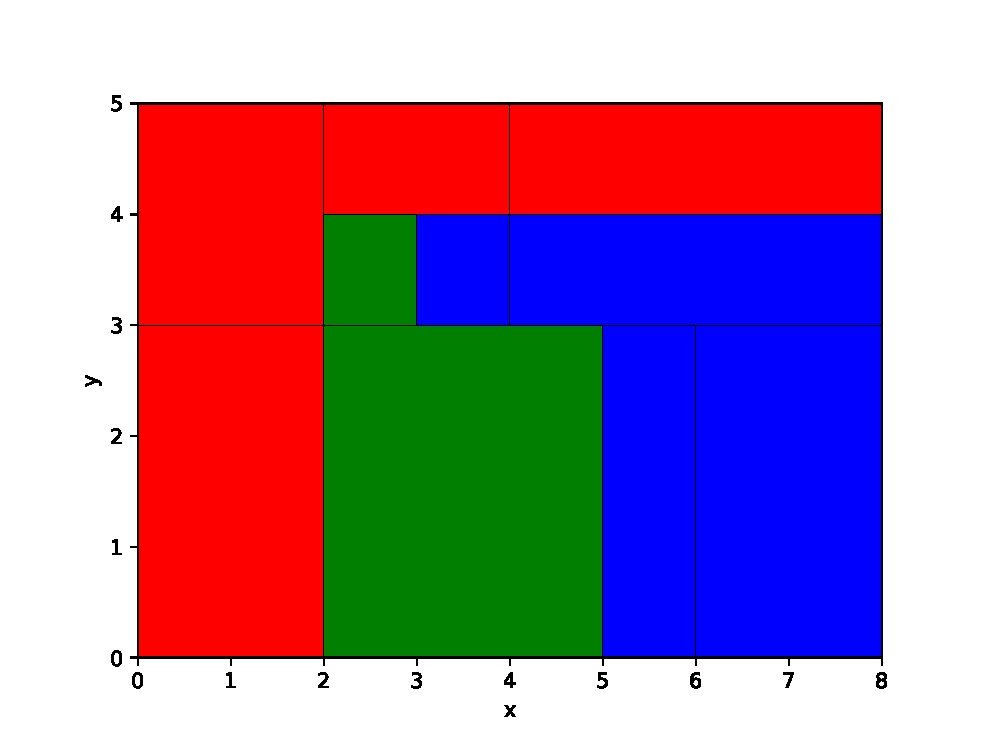
\includegraphics[width=.5 \textwidth]{complexExample2dVisual}%
  \label{fig:complexExample2dVisual}
  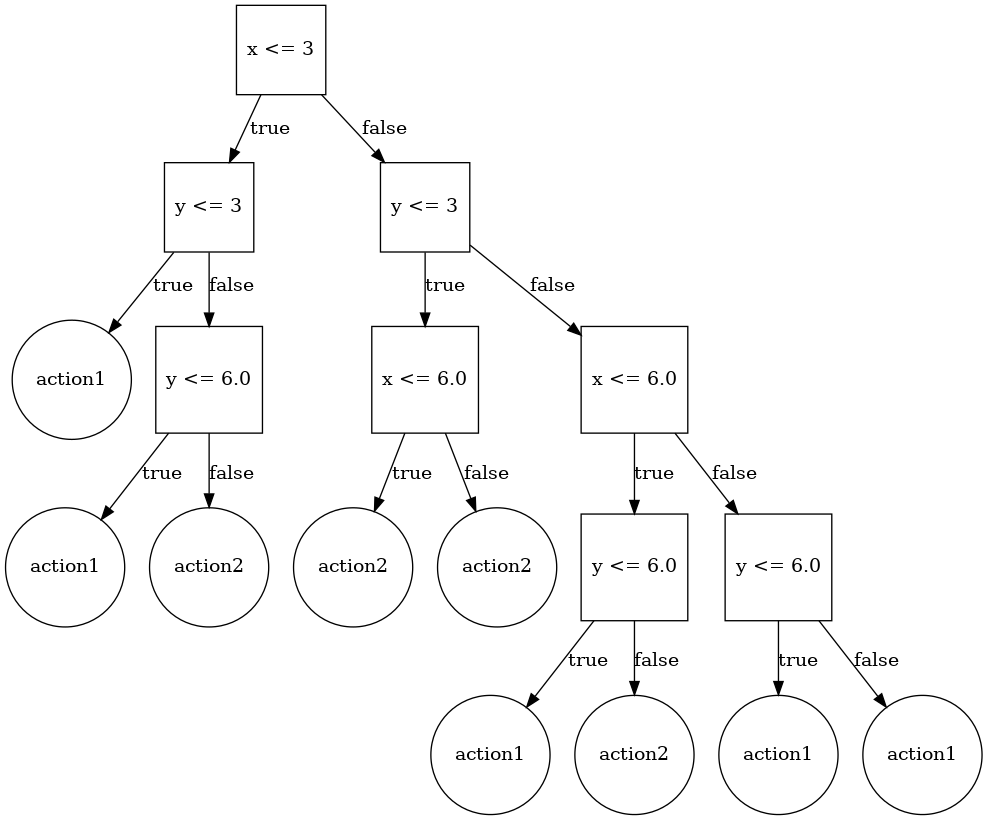
\includegraphics[width=.5 \textwidth]{complexExampleTree}%
  \label{fig:complexExampleTree}

  \caption{%
    Two representations of a strategy mapping states to actions. In
    \cref{fig:complexExample2dVisual} the strategy is represented as a
    partitioning with colors representing the assigned action. In
    \cref{fig:complexExampleTree} the strategy is given as a decision
    tree, which also induces the partitioning. For this small example, it is
    obvious to see that an equivalent state-action mapping could be achieved
    with fever regions/leaves.
  }%
  \label{fig:complexExample}
\end{figure}

However, we can (in this small toy example) easily see that we do not need 9
regions to represent this exact state-action mapping. For example, the two
regions given by $((3,0),(6,3))$ and $((6,0),(9,3))$, respectively, both assign
$action2$ as the optimal action, but this mapping would still be preserved if we
replaced those two regions with a larger one $((3,0),(9,3))$. After a little bit
of inspection, we can actually see here that we could represent the same
state-action mapping with a partitioning consisting of only 5 regions.

This example showcases how discretization techniques can easily end up with
redundancy in the partitioning. This can be very difficult to anticipate before
learning, especially since a very fine-grained discretization is typically
needed for the learning to capture essential information and details for the
strategy. Furthermore, for other learning techniques, such as the online
partitioning refinement scheme of \textsc{UPPAAL Stratego}~\cite{Manfred2019},
regions can be created on-the-fly, not be arranged in a straight grid and/or
vary in size, which can enhance the problem of redundancy.

We propose \textsc{MaxPartitions}, an algorithm that postprocesses a decision
tree inducing a partitioning of a state space in order to minimize the
partitioning by \textit{maximizing} the size of the individual regions (or
partitions). The output of \textsc{MaxPartitions} is a new partitioning, ie.\ a
list of regions with associated actions, which can then be arranged into a new
decision tree.


\subsection{Details of the algorithm}%
\label{sub:maxPartsDescription}

We write $\mathcal{T}_i$ for the (ascendingly) sorted list of bounds on
dimension $i$ in the policy given by the tree $\mathcal{T}$. The first bound in
the list is defined to be negative $\infty$ and the last is positive $\infty$.
By $\mathcal{T}_{i,j}$ we write the $j$th smallest bound on dimension $i$ for
each $j = 1, 2, \ldots, |\mathcal{T}_i|$. This can be precomputed as a matrix in
log-linear time by collecting and sorting the bounds on all branch nodes in
$\mathcal{T}$ and allows accessing $\mathcal{T}_{i,j}$ in constant time.
Further, in a slight abuse of notation, we define $\mathcal{T}_{i,
|\mathcal{T}_i| + 1}$ to be some \textit{sentinel} value representing that we
are outside the boundaries of dimension $i$. Correspondingly, we define a
sentinel action $\alpha$, and we say that $\mathcal{T}(s^p_{\mathcal{T}}) =
\alpha$ if and only if $\exists p_i \in p,\, p_i = |\mathcal{T}_i| + 1$.

Exploiting this notation, let $p$ be a $K$-dimensional vector of integers, such
that $p_i \leq |\mathcal{T}_i| + 1$ for all $i = 1,\ldots,K$, then we can define
a point at an intersection of bounds in $\mathcal{T}$ as $s^{p}_{\mathcal{T}} =
(\mathcal{T}_{1,p_1}, \mathcal{T}_{2,p_2}, \ldots, \mathcal{T}_{K,p_K})$. To
avoid cluttering the notation, will for the most part omit the subscript
$\mathcal{T}$ on $s^{p}_{\mathcal{T}}$. To make things clear, we will write $s$
to refer to an actual point in the state space of $\mathcal{T}$, ie.\ $s \in
\mathcal{S}$, and we will write $p$ to refer to a vector of integers
representing indicies of bounds in $\mathcal{T}$.

The algorithm (given in pseudo-code in Algorithm~\ref{alg:MaxPartitions}) works
by maintaining a pair $(p^{\min}, p^{\max}$), and iteratively incrementing
$p^{\max}$ in one dimension at a time until a region $\nu = (s^{p^{\min}},
s^{p^{\max}})$ cannot be expanded further. When this happens, the region is
added to a tree $\mathcal{T}_{track}$, which is used to track which areas of the
state space have been covered and to provide new a starting point for each
iteration of the algorithm. Expansion in dimension $i$ is disallowed if one of
the following three \textit{expansion rules} are violated by the expanded region
$\nu'$:

\begin{definition}[Expansion rules]\label{def:expansionRules}
    Let $\nu'$ be a candidate region for a new partitioning derived from
    $\mathcal{A}_{T}$. Then $\nu'$ is valid if it adheres to the following rules:

    \begin{enumerate}
        \item $\nu'$ does not have singular mapping in $\mathcal{T}$
        \item $\nu'$ intersects with one or more regions already in
            $\mathcal{T}_{track}$
        \item $\nu'$ intersects with a region $\nu_{o}$ in the original
            partitioning, such that the disjunction $\nu' \cap \nu_{o}$ cannot be
            described by a single region of the form $(s^{\min}, s^{\min})$
    \end{enumerate}
\end{definition}

\noindent The first two cases are directly related to the definition of the
problem, ie.\ the produced partitioning should respect $\mathcal{T}$ and only
have non-overlapping regions. The third case is required in order to guarantee
that in each iteration the algorithm on average will add \textit{at least} one
region from the original partitioning to the new partitioning. To see this,
consider \ldots\todo[inline]{Make an example to show}.


How do we determine this expansion? Let $(p^{\min}, p^{\max})$ define region in
the original partitioning (or potentially the remains of a region previously cut
in two). We then want to find a $\Delta_p \in \mathbb{Z}^K$ such that
$(p^{\min}, p^{\min} + \Delta_p)$ defines a region that follows the three
expansion rules and such that incrementing in any one dimension would result in
a violation. By definition, a valid value for $\Delta_p$ is when $\Delta_p =
p^{\max} - p^{\min}$, since this would just produce the original region. We are
therefore guaranteed to at least find this region. This gives rise to the
following definition.

% Let $p^{\min}$ be the result of popping the lexicographically smallest element
% of $\mathcal{P}$ (line 4). We can then define $s^{\min} = s^{p^{\min}}$ as the
% `lower left' corner in (or the origin of) a region $\nu = (s^{\min}, s^{\max})$
% where $s^{\max}$ is the point we want to determine, so that $\nu$ is maximized
% and has singular mapping in $\mathcal{T}$. By definition, $s^{\max} =
% s^{p^{\max}}$ satifies the singular mapping requirement for $p^{\max} =
% (p^{\min}_{1} + 1, \ldots, p^{\min}_{K} + 1)$, since no branch node in
% $\mathcal{T}$ splits on a predicate $c$ where $\mathcal{T}_{i,p^{\min}_{i}} < c
% < \mathcal{T}_{i,p^{\min}_{i} + 1}$ for any $i = 1, \ldots, K$.

% Finding a $p^{\max}$ that maximizes the region comes down to finding a vector
% $\Delta_{p} \in \mathbb{Z}^{K}$ so that $p^{\max} = p^{\min} + \Delta_{p}$. The
% definition of $\Delta_{p}$ is given below.

\begin{definition}[The expansion vector $\Delta_p$]
    Given $p^{\min} \in \mathbb{Z}^{K}$, a decision tree $\mathcal{T}$ over a
    $K$-dimensional space and a decision tree $\mathcal{T}_{track}$ of already
    found regions, $\Delta_{p} \in \mathbb{Z}^{K}$ is a vector such that for
    $p^{\max} = p^{\min} + \Delta_{p}$ the region $\nu =
    (s^{p^{\min}}_{\mathcal{T}}, s^{p^{\max}}_{\mathcal{T}})$ does not violate
    any of the expansion rules in Definition~\ref{def:expansionRules} and where
    for any other $\Delta'_p = (\Delta_{p_{1}}, \ldots, \Delta_{p_{i}} + 1,
    \ldots, \Delta_{p_{K}})$ this would not hold.
\end{definition}\label{def:deltaP}

\noindent A greedy approach to finding $\Delta_{p}$ starts with $\Delta_{p} =
p^{\max} - p^{\min}$, for some (remainder of a) region $\nu =
(s^{p^{\min}}_{\mathcal{T}}, s^{p^{\max}}_{\mathcal{T}})$. We then iteratively
increment a single dimension chosen non-deterministically untill the invariants
are violated.  Let $\mathbf{\hat{e}}_i$ denote the unit vector parallel to axis
$i$, such that $\Delta_{p} + \mathbf{\hat{e}}_i =
(\Delta_{p_1},\ldots,\Delta_{p_i} + 1,\ldots,\Delta_{p_K})$. At each increment,
we define a candidate region $\nu'$ from $p^{\min}$ and $p^{\max} = p^{\min} +
\Delta_{p}$ and check for singular mapping (Rule 1) and no overlap with regions
in $\mathcal{R}$ (Rule 2). If any of these two do not hold, we mark dimension
$i$ as exhausted, roll back the increment and continue with a new dimension not
marked as exhausted.

If Rule 3 is violated, the algorithm wil initiate an attempt at \textit{healing}
the candidate expansion, by continuing the expansion to the largest bound in
the expansion dimension of any of the broken regions. This way we try to see if
the violation can be overcome by simply expanding more aggressively. However,
care is required to ensure, that we can roll back this extra expansion if it did
not work (or if we inadverdently broke any of the other rules in the process).

When all dimensions have been
exhausted, $\Delta_{p}$ adheres to Defintion~\ref{def:deltaP}.

\begin{algorithm}[!ht]
    \caption{MaxPartitions}\label{alg:MaxPartitions}

    \begin{algorithmic}[1]
        \Require{%
            $\mathcal{T}$: A binary decision tree over the domain
            $\mathbb{R}^K$ inducing the partitioning $\mathcal{A}_{\mathcal{T}}$
        }
        \State{$\mathcal{T}_{track} \gets$ empty tree}
        \State{$\mathcal{R} \gets \{\}$}

        \While{$\mathcal{T}_{track}$ has unexplored regions}

            \State{%
                $(p^{\min}, p^{\max}) \gets$
                select region bounds of unexplored region
            }

            \State{%
                $\Delta_p \gets p^{\max} - p^{\min}$
            }

            \item[]
            \While{%
                not all dimensions have been exhausted
            }

                \State{%
                    $d \gets$ randomly select unexhausted dimension
                }
                \State{%
                    $\Delta_{p_{d}} \gets \Delta_{p_{d}} + 1$
                }

                \State{%
                    $\nu' \gets (s^{p^{\min}}_{\mathcal{T}}, s^{p^{\min} +
                    \Delta_p}_{\mathcal{T}})$
                }

                \item[]
                \If{%
                    $\nu'$ violates Rule 1 or 2
                    (Definition~\ref{def:expansionRules})
                }
                    \State{$\Delta_{p_{d}} \gets \Delta_{p_{d}} - 1$}
                    \State{mark $d$ as exhausted}

                \ElsIf{%
                    $\nu'$ violates Rule 3 (Definition~\ref{def:expansionRules})
                }
                    \State{attempt $healing$ in dimension $d$}
                \EndIf%

            \EndWhile%

            \item[]
            \State{%
                $\nu' \gets (s^{p^{\min}}_{\mathcal{T}}, s^{p^{\min} +
                \Delta_p}_{\mathcal{T}})$
            }
            \State{%
                \Call{Put}{$\mathcal{T}_{track},\, \nu'$}
            }
            \State{%
                $\mathcal{R} \gets \mathcal{R} \cup \{\nu'\}$
            }

        \EndWhile%

        \State{\textbf{return} $\mathcal{R}$}

    \end{algorithmic}

\end{algorithm}



\subsection{Analyzing the algorithm}%
\label{sub:maxPartsAnalysis}

In the following we provide an upper bound of the running time of
\textsc{MaxPartitions} and a proof of correctness.

\subsubsection{Running time}%
\label{sec:runningTime}

\subsubsection{Proof of correctness}%
\label{sec:proofCorrectness}

\subsection{From regions to decision tree}%
\label{sub:regionsToDT}

The output of the \textsc{MaxPartitions} algorithm is a list of regions with
associated actions. For this to be of any use, we need to construct a new
decision tree to represent these state-action pairs. To this goal, we face the
issue that it is not given (and in fact, very unlikely) that the suggested
partitioning can be perfectly represented by a decision tree, as this would
require the existence of enough `clean splits' (ie.\ predicates on some variable
that perfectly divides the regions into two sets with an empty intersection) to
arrange the entire set of regions.

Therefore, we suggest a brute-force algorithm that tries to separate the regions
as cleanly as possible. Let $\mathbf{R}$ be a list of regions and let $a_{\nu}$
be the action associated with the region $\nu = (s^{\min}, s^{\min})$. In the
following, we refer to $s^{\min}$ and $s^{\max}$ of a region $\nu$ by
$\nu_{\min}$ and $\nu_{\max}$ respectively, and to the value of a specific
dimension $i$ in one such boundary point as $\nu_{\min, i}$ or $\nu_{\max,i}$.

We iteratively create a branch node that splits $\mathbf{R}$ into two,
$\mathbf{R}_{low}$ and $\mathbf{R}_{high}$, based on a predicate function
$\rho(x) = x_i \le c$ with $c \in \mathbb{R}$ so that $\mathbf{R}_{low} = \{ \nu
\in \mathbf{R} \mid \rho(\nu_{\min}) \text{~is True} \}$ and $\mathbf{R}_{high}
= \{ \nu \in \mathbf{R} \mid \rho(\nu_{\max}) \text{~is False} \}$. When the
list only contains a single element $\nu$, we create a leaf node with action
$a_{\nu}$ and return.

The question is how to determine $\rho(x)$, more specifically which dimension
$i$ to predicate on and at which value $c$. Ideally, we want to split
$\mathbf{R}$ in two equally sized subsets and in a way that no single region
would have to occur in both, ie.\ we would like $\mathbf{R}_{low} \cap
\mathbf{R}_{high} = \emptyset$. For this we define an impurity measure
$I(\mathbf{R}_{low},\mathbf{R}_{high})$ that penalises the difference in size
between $\mathbf{R}_{low}$ and $\mathbf{R}_{high}$ and the size of the
intersection between the two. Let $abs(a)$ be the absolute value of $a$ and let
$|b|$ denote the size of a set $b$, then

\[
    I(\mathbf{R}_{low}, \mathbf{R}_{high})  = abs(|\mathbf{R}_{low}| -
    |\mathbf{R}_{high}|) + |\mathbf{R}_{low} \cap \mathbf{R}_{high}|
\]


Our brute-force way of finding the predicate that minimizes $I$ is to iterate
over the dimensions in $\mathcal{S}$ and for each dimension $i$ we sort the
regions according to their upper bound. Let $\mathbf{R}_i = \{ \nu^1, \nu^2,
\ldots, \nu^n \}$ be the list sorted according to the $i$ th dimension so that
for all $\nu^j, \nu^{j+1} \in \mathbf{R}_{i}$ it holds that $\nu^{j}_{\max,i} \le
\nu^{j+1}_{\max,i}$. If we then let $\rho(x) = x_i \le c$ with $c =
\nu^{j}_{\max,i}$ we have $|\mathbf{R}_{low}| = j$ and |$\mathbf{R}_{high}| = n
- j$. For determining the size of $\mathbf{R}_{low} \cap \mathbf{R}_{high}$ we
simply need to count the number of regions $\nu^{j+m}$ for $m = 1, 2, \ldots,
n-j$ whose lower bound is less than our predicate bound $c$, since these regions
will appear both in $\mathbf{R}_{low}$ (because then, by definition, $\rho(x) = x_i
\le c$ will be true for $x_i = \nu^{j+m}_{\min,i}$ and $c = \nu^{j}_{\max,i}$)
and in $\mathbf{R}_{high}$ (because our sorting ensures that for all
$\nu^{j},\nu^{j+m}$ it holds that $\nu^{j}_{\max,i} \le \nu^{j+m}_{\max,i}$).

Now we can write our impurity measure in terms of these quantities:

\[
    I(\mathbf{R}_{low}, \mathbf{R}_{high}) = abs(j - (n - j)) +
    \sum^{n}_{m=1} \mathbbm{1}(\rho(\nu^{j+m}_{\min})), \quad
    \text{for all }\nu^{j} \in \mathbf{R}_{i}
\]

\noindent
where $\mathbbm{1}$ is the indicator function, $\mathbf{R}_{i}$ is the list of
regions sorted according to upper bounds in dimension $i$ and $\mathbf{R}_{low}$ and
$\mathbf{R}_{high}$ are the subsets resulting from splitting on the predicate
function $\rho(x) = x_i \le c$ with $c = \nu^{j}_{\max,i}$ so that
$\mathbf{R}_{low} \subsetneq \mathbf{R}$, $\mathbf{R}_{high} \subsetneq
\mathbf{R}$ and $\mathbf{R} \supseteq \mathbf{R}_{low} \cup \mathbf{R}_{high}$.

Finding the best split, ie.\ the one that minimizes the impurity, is a $O(Kn^2)$
operation, as it requires a nested loop through all the regions for each
of the $K $dimensions (the nested loop being the final summation term over $m =
1, 2, \ldots, n - j$ for all $j = 1, 2, \ldots, n - 1$). In this work, we have
not attempted to find a faster implementation as we found that the size of
$\mathbf{R}$ obtained by using our \textsc{MaxPartitions} algorithm did not
cause performance issues.


